\documentclass[11pt,letterpaper]{article}

% Enable the inclusion of EPS-format graphics.
\usepackage{epsfig}
% Used to handle line spacing. Must be loaded before hyperref.
\usepackage{setspace}
% Clickable links.
\usepackage[bookmarks,colorlinks=true,linkcolor=blue,urlcolor=blue]{hyperref}
% Code listings via \lstlisting.
\usepackage{listings}
% Multirow table cell spanning.
\usepackage{multirow}
% Zero paragraph indent and non-zero paragraph separation.
\usepackage{parskip}
% Tables with flexible-width columns.
\usepackage{tabulary}
% Diagrams and stuff.
\usepackage{tikz}

% Set document fonts: Times as the default Roman font, Helvetica for
% sans-serif, Courier for teletype.
\renewcommand{\rmdefault}{ptm}
\renewcommand{\sfdefault}{phv}
\renewcommand{\ttdefault}{pcr}

% I want captions to have slightly smaller text and a bold label.
\usepackage[font=small,labelfont=bf]{caption}

% Customize formatting for code listings.
\lstset{
    basicstyle={\small\ttfamily}
}

% LaTeX' default line spacing is a little tight for my liking.
\setstretch{1.15}

\begin{document}

\title{
\includegraphics[width=0.75\textwidth]{logo.eps}\\
Module Architecture and Communictations}
\author{Samuel Coleman}
\date{\today}

% Turn off index link generation for the unnumbered title page so we don't get
% a warning about a missing page.
\hypersetup{pageanchor=false}
\begin{titlepage}

\maketitle
% Ditch the page styling (including page number) for the title page.
\thispagestyle{empty}

\end{titlepage}
% Having generated the page, we can turn index link generation back on.
\hypersetup{pageanchor=true}

\tableofcontents

\newpage

\section{Introduction}
\label{introduction}

``Online judge'' is a broad term for a software system which receives source
code submissions from users, compiles and runs them against a set of input
data, and judges the output of the submission against reference output. In
practice, online judges take several different forms: challenge archives like
UVa~Online~Judge\footnote{\url{http://uva.onlinejudge.org/}}; live competitions
like Google~Code~Jam\footnote{\url{http://code.google.com/codejam/}} and the
ACM~ICPC\footnote{\url{http://icpc.baylor.edu/}}; and hybrids like
Kattis\footnote{\url{https://open.kattis.com/}}. The Garrit project is an
attempt to design a modular architecture upon which any of these forms of
online judges can be implemented. A new project was started on the basis that
the most widely-used existing solutions were inappropriate for modification,
either because they are closed-source (for example,
PC\textasciicircum2\footnote{\url{http://www.ecs.csus.edu/pc2/}}), or because
they are specifically focused on providing the functionality required by only
one form of online judge
(e.g., DOMjudge\footnote{\url{http://www.domjudge.org/}}).

In addition to the capability descriptions provided in this document, Garrit
prescribes a common format for problem definitions. This format is described in
the document \emph{Garrit:~Problem~Definition~Format}.

Garrit also provides reference implementations for each system capability.
The source code repositories for these projects are accessible via the
Garrit~GitHub~organization\footnote{\url{https://github.com/Garrit/}}, and are
described in the document \emph{Garrit:~Reference~Implementations~Explained}.

\section{Design}
\label{design}

Garrit defines a microservices-oriented approach to infrastructure modularity.
A system is comprised of a collection of components, each providing one or more
of five \emph{capabilities}. These components communicate with each other
through JSON-encoded messages exchanged over HTTP via REST-like API endpoints
exposed by the components. For more details on inter-component communication,
see the \nameref{endpoints} section.

\begin{figure}[h]
\centering
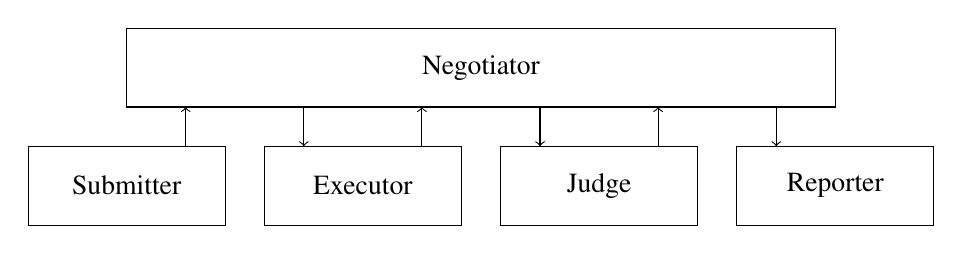
\begin{tikzpicture}
% Negotiator
\draw (1.25,1.5) rectangle (10.25,2.5) node[midway] {Negotiator};
% Submittor and connecting lines
\draw (0,0) rectangle (2.5,1) node[midway] {Submitter};
\draw[->] (2,1) -- (2,1.5);
% Executor and connecting lines
\draw (3,0) rectangle (5.5,1) node[midway] {Executor};
\draw[->] (3.5,1.5) -- (3.5,1);
\draw[->] (5,1) -- (5,1.5);
% Judge and connecting lines
\draw (6,0) rectangle (8.5,1) node[midway] {Judge};
\draw[->] (6.5,1.5) -- (6.5,1);
\draw[->] (8,1) -- (8,1.5);
% Reporter and connecting lines
\draw (9,0) rectangle (11.5,1) node[midway] {Reporter};
\draw[->] (9.5,1.5) -- (9.5,1);
\end{tikzpicture}
\caption{A visual representation of Garrit module capabilities and their
connections.}
\end{figure}

Each capability represents a separate stage in the process of receiving and
evaluating a user submission:

\begin{itemize}
\item Submitters receive problem submissions from users, perhaps by way of a
web interface or client program, and act as an entry point into the rest of the
system.
\item Executors perform actions upon problem submissions: compilation and
execution, static analysis, etc.
\item Judges process the output of executors to determine a score for problem
submissions. This could be comparison of program output to a ``known good''
output, or simply reformatting program output.
\item Reporters make judging results available to end users. They may be
integrated into the submission interface, provided over e-mail, etc.
\item Negotiators provide a messaging backbone upon which all other components
can communicate. Instead of talking directly to each other, components address
the negotiator causing the it to instruct another component to perform some
task.
\end{itemize}

A functional environment will consist of a collection of one or more components
(typically more) providing at least one instance of every type of capability,
with the exception of negotiation, which may only be provided by one component.

\subsection{Submitter}
\label{design-submitter}

The submitter and \hyperref[design-reporter]{reporter} serve as the user
interface to a Garrit environment. As such, they are the most fluidly-defined
component. Providing they can correctly communicate with the negotiator, they
may be implemented in any one of a number of different forms: a web interface,
a desktop client, a command line utility, an IRC bot, etc. Typically, the
submitter and reporter will be tied together, conceptually if not concretely.

\subsection{Executors and Judges}
\label{design-executor-judge}

Executors and judges, while performing different operations, both essentially
act as ``filter programs'': they take some input data (the problem submission),
perform some processing (compilation and execution or judging), and output
other data (program execution results or judging conclusions). This gives
plenty of implementation flexibility: requests can be handled serially, in
parallel by multiple worker threads, batched (if there ever were a problem
to take advantage of such a mechanism), or whatever else you can think of.

As the executor is, by definition, relegated to evaluating untrusted,
user-submitted programs, some means of isolation for the execution environment
is necessary. Implementations should be very careful in protecting the secret
input data of problem sets, and should at the very least restrict the network
access of submitted programs.

The judge could approach the task of comparing the case output to the execution
output from a couple of different angles. The most straightforward is an exact
file comparison, which rapidly falls apart in the face of problems with
subjective output or multiple correct output options. While these problems
can often be minimized through careful construction of the problem definition,
it is still nice to have options. As such, a more flexible judge might support
judging output consisting of one regular expression per line against which
submission output can be matched.

\subsection{Reporter}
\label{design-reporter}

Reporters, upon receiving judging output, are expected to provide some means by
which users can access the judging results. This is also a very logical point
at which to store results in a database for later access, assuming a
loosely-coupled system wherein the reporter and negotiator are not aware of
each other.

There are many ways in which results could be reported. As with submitters,
viable options include a web interface or a desktop client, and indeed, both
reporting and submission capabilities could be built into the same component.

\subsection{Negotiator}
\label{design-hub}

The negotiator ties all other components together. Modules in a system do not
pass messages directly to each other, but rather indicate to the negotiator
that they have finished a task and that successive modules should be notified.
By introducing an intermediary to handle inter-module messaging, two benefits
are realized: modules are forced to remain compliant with the messaging
specification, and more complex message routing may be accomplished. For
example, a system may have multiple executors, one for each supported language;
the negotiator, upon receiving a submisison, determines which executor(s) are
capable of receiving the submission, and relays it appropriately.

A negotiator ought to be configured with a list of all components with which it
shall communicate. Because components report which capabilities they provide,
it is not necessary for such a configuration to ``bin'' lists of components per
capability. In fact, given the possibility of components providing multiple
capabilities, it would be preferable if it did not.

On startup, a negotiator should interrogate all configured components to
understand which capabilities are available, and to build a map of which
languages and problems can be processed by which components. It would be
strongly preferable for the negotiator to provide an interface by which this
task can be performed again during normal operation to save restarting the
whole negotiator in the event of the arrival of new problem definitions or
languages. (Consider a classroom environment where new problems may be
introduced over the course of a semester.)

Upon receiving a submission, the negotiator will assign it a unique integer
identifier before passing it on to waiting executors. If an negotiator
distributes a problem to multiple executors, it should collate results destined
for the same judge. That is, a judge should not see more than one set of
execution data for the same submission ID unless that submission is being
reevaluated. The simplest way to accomplish this may be counting the number of
executors to which a submission is sent, and not sending any execution results
for that submission on to any judging components until the number of execution
results equal to the number of executors involved have been collected.

Similarly, the results from multiple judges should be collated before they are
exposed to any reporters. A reporter should not see more than one set of
judging results for the same submission ID unless that submission is being
reevaluated.

Other components will report back to the negotiator with errors should any
occur during processing. The negotiator may provide an administrative interface
allowing administrators to resubmit failed submissions to the component in
which the failure occurred.

\section{Communication Endpoints}
\label{endpoints}

Communication between components is accomplished through the exchange of
JSON-encoded messages over HTTP connections. Each component which receives data
from within the system to do its job (i.e., every component implementing any
capability other than that of a submitter) exposes REST endpoints to which the
negotiator can connect to deliver messages.

The formats of messages exchanged between components is noted in the
\nameref{formats} section.

In all cases, the component must respond with an appropriate HTTP error code.
Unless otherwise noted, all calls invoke asynchronous actions and response
bodies are optional.

Only the minimal set of endpoints is defined here. Implementations may add
custom endpoints as long as they do not conflict with this specification.

\subsection{Common Endpoints}
\label{endpoints-common}

\subsubsection{\texttt{/status}}

\emph{Verb: \texttt{GET}; body: \nameref{formats-status}}

Provides some metrics and capabilities information from a running component.

A request made to this endpoint does not require any body. The response
describes the status of the component, and which capabilities it provides.

\subsection{Submitter Endpoints}
\label{endpoints-sub}

This specification defines no endpoints for submitters.

\subsection{Executor Endpoints}
\label{endpoints-exec}

\subsubsection{\texttt{/execute}}

\emph{Verb: \texttt{POST}; body: \nameref{formats-reg-sub}}

Enqueue a submission for compilation and execution.

\subsection{Judge Endpoints}
\label{endpoints-judge}

\subsubsection{\texttt{/judge}}

\emph{Verb: \texttt{POST}; body: \nameref{formats-exec}}

Enqueue an execution for judgement.

\subsection{Reporter Endpoints}
\label{endpoints-report}

\subsubsection{\texttt{/report}}

\emph{Verb: \texttt{POST}; body: \nameref{formats-judge}}

Release judging results for user consumption.

\subsection{Negotiator Endpoints}
\label{endpoints-hub}

\subsubsection{\texttt{/submit}}

\emph{Verb: \texttt{POST}; body: \nameref{formats-sub}}

Introduce a submission into the system for evaluation. The submission may not
be evaluated immediately, but will be queued for evaluation.

The negotiator will respond to this request with a \nameref{formats-reg-sub}
populated with the newly-generated unique ID for the submission.

\subsubsection{\texttt{/execute/:id}}

\emph{Verb: \texttt{POST}; body: \nameref{formats-exec}}

Called by \hyperref[design-executor-judge]{executors} after having evaluated a
submission.

The \texttt{:id} parameter is the unique ID of the executed submission.

\subsubsection{\texttt{/judge/:id}}

\emph{Verb: \texttt{POST}; body: \nameref{formats-judge}}

Called by \hyperref[design-executor-judge]{judges} after having evaluated an
execution.

The \texttt{:id} parameter is the unique ID of the judged submission.

\subsubsection{\texttt{/error/:id}}

\emph{Verb: \texttt{POST}; body: \nameref{formats-error}}

Called by any component other than submitters upon encountering an error
processing a submission.

The \texttt{:id} parameter is the unique ID of the submission in error.

\section{Message Formats}
\label{formats}

\subsection{Submission}
\label{formats-sub}

A \emph{submission} is the basic representation of the source code submission
fed into the system by the user. An example of this basic structure as a JSON
document can be seen in \autoref{formats-sub-listing}.

As a submission progresses through the chain of components, data is
progressively added to the representation of the submission, and no existing
data is redacted.

Upon its initial introduction into the system, a submission has the following
fields:

\nopagebreak
\begin{tabulary}{\textwidth}{ | l | l | L | }
    \hline
    \textbf{Key} & \textbf{Type} & \textbf{Value} \\
    \hline
    \texttt{language} & string & The language in which the submission is
        written. \\
    \hline
    \texttt{problem} & string & The name of the problem for which this
        submission is a solution. \\
    \hline
    \texttt{files} & array & An array of objects, each describing a file
        required for execution. \\
    \hline
    \texttt{entryPoint} & string & The name of the entry point of the submitted
        program, as required by the language (e.g., the name of the class
        containing a main method for Java programs). \\
    \hline
\end{tabulary}

Submission files are described as follows:

\nopagebreak
\begin{tabulary}{\textwidth}{ | l | l | L | }
    \hline
    \textbf{Key} & \textbf{Type} & \textbf{Value} \\
    \texttt{filename} & string & The name of the file. Directory names are
        permitted (e.g., \texttt{ca/acadiau/socs/Example.java}), but paths must
        be relative and may not traverse above the initial directory (e.g., may
        not start with \texttt{/}, may not perform traversals such as
        \texttt{foo/../../bar}, etc.). \\
    \hline
    \texttt{contents} & string & The contents of the file as a Base64-encoded
        string. \\
    \hline
\end{tabulary}

\begin{figure}
\begin{lstlisting}
{
    "language": "",
    "problem": "",
    "files": [
        {
            "filename": "",
            "contents": ""
        }
    ],
    "entryPoint": ""
}
\end{lstlisting}
\caption{The basic structure of a submission.}
\label{formats-sub-listing}
\end{figure}

\subsection{Registered Submission}
\label{formats-reg-sub}

A \emph{registered submission} is the intermediary form of
\hyperref[formats-sub]{submission} produced by the negotiator immediately
after assigning it a numeric identifier. It differs from submissions in that it
provides a field for the identifier.

Registered submissions add the following fields to submissions:

\nopagebreak
\begin{tabulary}{\textwidth}{ | l | l | L | }
    \hline
    \textbf{Key} & \textbf{Type} & \textbf{Value} \\
    \hline
    \texttt{id} & integer & The ID of the submission, as generated by the
        negotiator. \\
    \hline
\end{tabulary}

\subsection{Execution}
\label{formats-exec}

An \emph{execution} represents the results of an
\hyperref[design-executor-judge]{executor} having compiled and executed a
registered submission against a problem set. The following fields are added to
the object:

\nopagebreak
\begin{tabulary}{\textwidth}{ | l | l | L | }
    \hline
    \textbf{Key} & \textbf{Type} & \textbf{Value} \\
    \hline
    \texttt{cases} & array & An array of objects, each representing the outcome
        of a problem case. \\
    \hline
\end{tabulary}

The format of execution case results is as follows:

\nopagebreak
\begin{tabulary}{\textwidth}{ | l | l | L | }
    \hline
    \textbf{Key} & \textbf{Type} & \textbf{Value} \\
    \hline
    \texttt{name} & string & The name of the case. \\
    \hline
    \texttt{runtime} & integer & The time consumed in seconds while evaluating
        the case. \\
    \hline
    \texttt{output} & string & A Base64-encoded string representation of the
        output of the submission for the case input. \\
    \hline
\end{tabulary}

\subsection{Judgement}
\label{formats-judge}

A \emph{judgement} represents the results of a
\hyperref[design-executor-judge]{judge} having evaluated an
\hyperref[formats-exec]{execution} for correctness. No fields are added to
the submission object, but the following fields are added to the execution case
object:

\nopagebreak
\begin{tabulary}{\textwidth}{ | l | l | L | }
    \hline
    \textbf{Key} & \textbf{Type} & \textbf{Value} \\
    \hline
    \texttt{value} & integer & The numeric value of the judgement. \\
    \hline
    \texttt{valueMin} & integer & This and \texttt{valueMax} serve to provide
        context for the judgement value. For a boolean judgement, these values
        could be given as \texttt{0} and \texttt{1}, with the \texttt{value}
        given as \texttt{0} or \texttt{1}. Or, for a judgement given as a
        percentage, the values could be given as \texttt{0} and \texttt{100}.
        \\
    \hline
    \texttt{valueMax} & integer & See \texttt{valueMin}. \\
    \hline
    \texttt{notes} & string & Free text describing the result.
        \emph{Optional.} \\
    \hline
\end{tabulary}

\subsection{Error}
\label{formats-error}

In the event of an error occurring at any stage during submission processing,
the component encountering the error ceases to process the erroneous submission
and reports the failure back to the negotiator. In turn, the negotiator informs
\hyperref[design-reporter]{reporters} of the failure. In both of these
exchanges, the same message format is used:

\begin{tabulary}{\textwidth}{ | l | l | L | }
    \hline
    \textbf{Key} & \textbf{Type} & \textbf{Value} \\
    \hline
    \texttt{id} & integer & The unique ID of the submission causing the error.
        If the error occurred while making the initial submission, this field
        will receive the ID that the negotiator would have otherwise given the
        submission. Otherwise, the value of this field will replicate the ID of
        the registered submission. \\
    \hline
    \texttt{stage} & string & The stage of processing at which the error
        occurred. In the case of a component self-reporting a failure, this
        will be the capability of the component itself; otherwise, the
        negotiator will indicate the capability type of the component which
        caused the error.
        \newline
        \newline
        May be one of \texttt{submittor}, \texttt{executor}, \texttt{judge},
        \texttt{reporter}, or \texttt{negotiator}. \\
    \hline
    \texttt{type} & string & The type of error which has occurred. See the
        table below for details. \\
    \hline
    \texttt{message} & string & An error message. \emph{Optional.} \\
    \hline
    \texttt{submission} & object & The submission causing the error. This
        should be either a \hyperref[formats-sub]{submission},
        \hyperref[formats-reg-sub]{registered submission},
        \hyperref[formats-exec]{execution}, or
        \hyperref[formats-judge]{judgement}. \\
    \hline
\end{tabulary}

The following error types are possible:

\begin{tabulary}{\textwidth}{ | l | L | }
    \hline
    \textbf{Error Type} & \textbf{Description} \\
    \hline
    \texttt{E\_OTHER} & An error which doesn't fit into any of the other
        defined categories. \\
    \hline
    \texttt{E\_INTERNAL} & An error caused by an internal malfunction of the
        component. \\
    \hline
    \texttt{E\_COMPILATION} & A failure during submission compilation. \\
    \hline
    \texttt{E\_RUNTIME} & A failure occurring during submission execution. \\
    \hline
    \texttt{E\_JUDGING} & A failure while judging the submission. \\
    \hline
\end{tabulary}

\subsection{Status}
\label{formats-status}

Each component must provide a \hyperref[endpoints-common]{status} endpoint
providing insight into its state and availability. The object representing the
status must provide the following fields:

\begin{tabulary}{\textwidth}{ | l | l | L | }
    \hline
    \textbf{Key} & \textbf{Type} & \textbf{Value} \\
    \hline
    \texttt{name} & string & A name which uniquely identifies the component
        within the environment. \\
    \hline
    \texttt{uptime} & integer & The number of seconds for which the component
        has been running. \\
    \hline
    \texttt{provides} & object & Insight into the capabilities provided by the
        component. See below for details on possible keys and their associated
        values. \\
    \hline
\end{tabulary}

\end{document}